\chapter{What is the Semantic Web?}
\label{ch1}
% \chapterauthor{Sally Smith, Joe Jones}        % For contributed chapters.

This book is about something we call the Semantic Web. From the name, you can probably guess that it is related somehow to the World Wide Web (WWW) 
and that it has something to do with semantics. Semantics, in turn, has to do with understanding the nature of meaning, but even the word 
semantics has a number of meanings. In what sense are we using the word semantics? And how can it be applied to the Web?\\
This book is for a working ontologist. That is, the aim of this book is not to motivate or pitch the Semantic Web but to provide the tools 
necessary for working with it. Or, perhaps more accurately, the World Wide Web Consortium (W3C) has provided these tools in the forms of 
standard Semantic Web languages, complete with abstract syntax, model-based semantics, reference implementations, test cases, and so forth. But these are 
like any tools - there are some basic tools that are all you need to build many useful things, and there are specialized craftsman’s 
tools that can produce far more specialized outputs. Whichever tools are needed for a particular task, however,  one  still  needs  to  
understand  how  to  use  them.  In the hands of someone with no knowledge, they can produce clumsy, ugly, barely functional output, but 
in the hands of a skilled craftsman, they can produce works of utility, beauty, and durability. It is our aim in this book to describe 
the craft of building Semantic Web systems. We go beyond only providing a coverage of  the  fundamental  tools  to  also  show  how  
they  can  be  used  together  to  create  semantic models, sometimes called \textit{ontologies} or \textit{vocabularies}, that are 
understandable, useful, durable, and perhaps even beautiful.1


\section{What is a web?}
\label{ch01.sec11.1}

The Web architecture was built by standing on the shoulders of giants. Writing in \emph{The Atlantic} magazine in 1945
\cite{Bush45aswe},
Vannevar Bush identified the problems in managing large collections of documents the links 
we make between them. Bush’s proposal was to consider this as a scientific problem, and among the ideas he proposed was the one of 
externalizing and automating 
the storage and management of association links we make in our readings. He also illustrated his ideas with an imaginary device he called 
the \textit{Memex} (‘memory extension”) that would assist us in studying, linking and remembering the documents we work with and the association 
links we weave between them. Twenty years later, Ted Nelson quoted \textit{As We May Think} and proposed using a computer to implement the idea, 
using hypertext and hypermedia structures to link parts of documents together. In the late sixties, Douglas Engelbart and the Augment project 
provided the mouse and new means of interaction and applied them in particular to hypertext editing and browsing. The beginning of the 
seventies brought the work of Vinton Cerf and the emergence of the Internet, which connected computers all around the world. By the 
end of the eighties, Tim Berners-Lee was able to stand on the shoulders of these giants when he proposed a new breakthrough: an architecture 
for distributing hypermedia on the internet, which we now know as the World Wide Web. The Web provides a hyptertext infrastructure that links 
documents across the internet, i.e., connecting documents that are not on the same machine. And so the Web was born. The Web architecture 
includes two important parts: Web clients, the most well-known being the Web browser, and  Web servers, that serve documents and data 
to the clients whenever they require it. For this architecture to work, there has to be three initial essential components. 
First, addresses that allow us to identify and locate the document on the Web; second, communication protocols that allow 
a client to connect to a server, send a request and get an answer; and third, representation languages to describe the 
content of the pages, the documents that are to be transferred. These three components comprise a basic Web architecture, 
which the Semantic Web standards, which we will describe later in this book, extend in order to publish semantic data on the Web.

The idea of a web of information was once a technical idea accessible only to highly trained, elite information professionals: 
IT administrators, librarians, information architects, and the like. Since the widespread adoption of the World Wide Web, 
it is now common to expect just about anyone to be familiar with the idea of a 
web of information that is shared around the world. Contributions to 
this web come from every source, and every topic you can think of is covered.

Essential to the notion of the Web is the idea of an open community: anyone can contribute their ideas to the whole, 
for anyone to see. It is this openness that has resulted in the astonishing comprehensiveness of topics covered by the 
Web. An information ``web'' is an organic entity that grows from the interests and energy of the communities that 
support it. As such, it is a hodgepodge of different analyses, presentations, and summaries of any topic that 
suits the fancy of anyone with the energy to publish a web page. Even as a hodgepodge, the Web is pretty useful. 
Anyone with the patience and savvy to dig through it can find support for just about any inquiry that interests 
them. But the Web often feels like it is a mile wide but an inch deep. How can we build a more integrated, 
consistent, deep Web experience?


\section{Communicating with Data}
\label{webdata}
Suppose you are thinking about heading to your favorite local restaurant, 
\emph{Copious}, so you ask your automated personal assistant, "what are the hours for
Copious?"  Your assistant replies that it doesn't have the hours for Copious.  
So you go to a web page, look them up, and find right there, next to the 
address and the daily special, the opening. hours.  How could the web master
at Copious have told your assistant about what was on the web page?   Then you
wouldn't just be able to find out the opening hours, but also the daily special. 

 
Suppose you consult a web page, looking for a major national park, and
you find a list of hotels that have branches in the vicinity of the
park. You don't find your favorite hotel, Mongotel.  But you go to their 
website, and find a list of their locations.  Some of them are near the park. 
Why didn't the park know about that?   How could Mongotel have published its
locations in a way that the park could have found them? 

Going one step further, you want to figure out which of your hotel locations is 
nearest to the park.  You have the address of the park, and the addresses of 
your hotel locations.  And you have any number of mapping services on the web. 
One of them shows the park, and some hotels nearby, but they don't have all the Mongotel locations. 
So you spend some
time copying and pasting the addresses from the Mongotel page to the map, and you 
do the same for the park.  You think to yourself, ``Why should I be the one
to copy this information from one page to another? Whose job is it to keep this
information up to date?''  Of course, Mongotel would be very happy if the data on 
the mapping page would be up to date.  What can they do to make this happen? 


Suppose you are maintain an amateur astronomy resource, and you have a section about our solar system. 
You organize news and other information about  objects in the solar system: Stars (well,
there's just one of those), planets, moons, asteroids, and comets. 
Each object has its own web page, with photos, 
essential information (mass, albedo, distance from the sun, shape, size,
what object it revolves around, period of rotation, period of
revolution, etc.), and news about recent findings, observations, etc. . 
You source your information from various places; the reference data comes from the 
International Astronomical
Union (IAU), the news comes from a number of feeds.  


One day, you read in the newspaper that the (IAU) has decided that Pluto, 
which up until 2006 was considered a
planet, should be considered a member of a new category called a ``dwarf
planet''!   You will need to update your web pages, since not only has the 
information on some page changed, but so has the way you organize it; in addition 
to your pages about planets, moons, asteroids, etc., you'll need a new page about 
``dwarf planets''.    But your page about planets takes its information from the 
IAU already.  Is there something they could do, so that your planet page would 
list the correct eight planets, without you having to re-organize anything? 

You have an appointment with your dentist, and you want to look them up.  You remember 
where the office is (somewhere on East Long street) and 
the name of the dentist, but you don't remember the name of the clinic.  So you look for dentists
on Long street.   None of them ring a bell.   When you finally find their web page, you 
see that they list themselves as "oral surgeons", not dentists.  Who's job is it to 
know all the ways a dentist might list themselves? 

You are a scientist researching a particular medical condition, whose metabolic process
is well understood.  From this process, you know a number of compounds that play a role
in the process.  Researchers around the world have published experimental results about
organic compounds linked to human metabolism.  Have any experiments been done about 
any of the compounds you are interested in?  What did they measure?  How can the scientists of 
the world publish their data so that you can find it? 

Tigerbank lends money to homeowners in the form of mortgages, as does Makobank; some of them
are at fixed interest rates, and some float according to a published index. A clever 
financial engineer puts together a deal where one of Tigerbank's fixed loan payments
are traded for one of Makobanks' floating loan payments.  These deals make sense for people who 
want to mitigate the different risk profiles of these loans.  Is this sort of swap a good 
deal or not?   We have to compare the terms of Tigerbank's loan with those of Makobank's loan.  
How can the banks describe their loans in terms that participants can use to compare them?


What do these examples have in common?  In each case, someone has knowledge of some thing that 
they want to share.  It might be about their business (hours, daily special, locations, business category), or 
scientific data (experimental data about compounds, the classification of a planet), or information 
about complex instruments that they have built (financial instruments).   It is in the best interests
of the entities with the data to publicise it to a community of possible consumers, but the 
data is too idiosyncratic, or too detailed, or just too complex to simply publicize by writing a description
of it.   In fact, it is so much in their interest to get this data out, that they are willing to 
put some effort into finding the right people who need their data.  


\subsection{Social Data}

A special case of the desire to share data is social networking.  Billions of 
people share data about their lives on a number of social websites, including 
their personal lives as well as their professional lives.  It is worth their 
while to share this data, as it provides ways for them to find new friends, keep
in touch with old friends, find business connections, and many other advantages. 

Social and professional networking is done in a non-distributed way.  Someone 
who wants to share their professional or personal information signs up for a web 
service (common ones today include Facebook and LinkedIn.  Others have come and gone,
and more will probably appear as time goes on), creates an account that they have control of, and 
they provide data, in the 
form of daily updates, photos, tags of places they've  been and people they've been with, 
projects they have started or completed, jobs they have done, etc.  This data is 
published for their friends and colleagues, and indeed perfect strangers, to 
search and view. 

In these cases, the service they signed up for owns the data, and can use it for 
various purposes.  Most people have experienced the eerie effect of having mentioned
something in a social network, only to find a related advertisement appear on their
page the following day. 

Advertising is a lucrative but mostly harmless use of this data.  In 2018, it 
was discovered that data from Facebook for millions of users had been used 
to influence a number of high-profile elections around the world, including the 
US presidential election of 2016 and so-called "Brexit" referendum in the
UK\cite{cambridge2018}.  Many
users were surprised that this could happen; they shared their data in a centralized
repository over which they had no control.  

This example shows the need for a balance of control - yes, I want to share my
data in the examples of Section~\ref{webdata}, and I want to share it with 
certain people but not with others (as is the case in this section). How can
we manage both of these desires?  This is a problem of distributed data; I need
to keep data to myself if I want to control it, but it has to connect to data
around the world to satisfy the reasons why I publish it in the first place. 


\subsection{Learning from Data}

Data Science has become one of the most productive ways to make business predictions,
and is used across many industries, to make predictions for marketing, demand, 
evaluation of risk, and many other settings in which it is productive to be 
able to predict how some person will behave or how well some product will perform. 

Banking provides some simple examples.  A bank is in the business of making loans, 
sometimes mortgages for homeowners, or automobile loans, small-business loans etc. 
As part of the loan application process, the bank learns a good deal about the 
borrower.  Most banks have been making loans for many decades, and have plenty of data
about the eventual disposition of these loans (e.g., were they defaulted?  Did they pay off 
early?  Were they refinanced?) By gathering large amounts of this data, machine learning techniques can 
predict the eventual disposition of a loan based on information gathered at the outset. 
This, in turn, allows the bank to be more selective in the loans it makes, allowing it 
to be more effective in its market. 

This basic approach has been applied to marketing (identifying more likely sales leads), product development
(identifying which features will sell best), customer retention (identifying problems before 
they become too severe to deal with), medicine (identifying diseases based on patterns in 
images and blood tests), route planning (finding best routes for airplanes), sports (deciding which 
players to use at what time), and many other high-profile applications. 

In all of these cases, success relied on the availability of meaningful data.  In the case of marketing, sales and 
manufacturing applications, the data comes from a single source, that is, the sales behavior of the customers 
of a single company.  In the case of sports, the statistical data for the sport has been normalized
by sports fans for generations.  The data is already aligned into a single representation. This is an important
step that allows machine learning algorithms to generalize the data. 

The only example in this list where the data is distributed is medicine, where diagnoses come 
from hospitals and clinics from around the world.  This is not an accident; in the case of medicine, 
disease and treatment codes have been in place for decades to align data from multiple sources. 

How can we extend the successful example of machine learning in medicine, to take 
our machine learning successes from the enterprise level to the industrial level in other industries? 
We need a way to link together data that is distributed throughout an industry. 


\section{Distributed data}



In the restaurant example, we had data (opening hours) published so that they 
can be read by the human eye, but our automated assistant can't read them.  One solution 
would be to develop sophisticated algorithms that can read web pages and figure out
the opening hours based on what it sees there.  But the restaurant owner knows the hours, 
and wants prospective patrons to find them, and for them to be accurate.  Why should 
a restaurant owner rely on some third party to facilitate communication to their customers?  

A scientific paper that reports on an experimental finding has a very specific audience;
other researchers who need to know about that compound and how it reacts in certain circumstances. 
It behooves both the author and the reader to match these up.  Once again, the author does not
want to rely on someone else to communicate their value. 

This story repeats at every level; a bank has more control over its own instruments if it 
can communicate their terms in a clear and unambiguous way (to partners, clients or regulators)
The IAU's charter is to keep the astronomical community informed about developments in 
observations and classifications.  Dentists want their patients to be able to find their clinics. 

The unifying theme in all of these examples is a move from a presentation of information 
for a specific audience, requiring interpretation from a human being to an exchange of data
between machines.  Instead of relying on human intuition just in the interpretation of the
data, we meet half-way; have data providers make it easier to consume the data.  We take advantage of 
the desire to share data, to make it easier to consume. 

Instead of thinking of each data source as a single point that is communicating one thing 
to one person, it is a multi-use part of an interconnected network of data.   Human users and 
machine applications that want to make use of this data collaborate with data providers, taking 
advantage of the fact that it is profitable to share your data.

\subsection{A distributed web of data}




The Semantic Web takes this idea one step further, applying it to the
Web as a whole. The Web architecture we are familiar with supports a distributed
network of hypertext pages that can refer to one another with global links
called Uniform Resource Locators (URLs). 

The main idea of the Semantic Web is to support a distributed Web at the
level of the data rather than at the level of the presentation. Instead
of just having one web page point to another, one data item can point to
another, using the same global references that web pages use -- Uniform
Resource Identifiers (URIs).   When Mongotel publishes information about its hotels and
their locations, or when Copious publishes its opening hour, they don't
just publish a human-readable presentation
of this information but instead a distributable, machine-readable
description of the data. 

The Semantic Web faces the problem of distributed data head-on.  Just as 
the hypertext web changed how we think about availability of documents, 
the Semantic Web is a radical way of thinking about data.  At first blush,
distributed data seems easy; just put databases all over the web (data on the web).
But in order for this to act as a distributed \emph{web of data},  we have 
to understand the dynamics of sharing data among multiple stakeholders across
a diverse world.   Different sources can agree or disagree, and data  can be 
combined from different sources to gain more insight about a single topic. 

Even within a single company, data can be considered as a distributed resource. Multiple
data bases, from different business units, or from parts of the business that 
were acquired through merger or corporate buy-out, can be just as disparate as 
sources from across the web.  Distributed data means that the data comes from 
multiple stakeholders, and we need to understand how to bring the data together
in a meaningful way.

Broadly speaking, data makes a statement that relates one thing to another, in some 
way.  Copious (one thing) opens (a way to relate to something else) at 5:00pm (another
thing, this time a value).  They serve (another way to relate to something) Chicken 
and Waffles (this time, a dish), which itself is made up (another way to relate) of
some other things (chicken, Waffles, and a few others not in its name, like 
maple syrup).  Any of these things can be represented at any source in a distributed web of data. 
The data model that the Semantic Web
uses to represent this distributed web of data is
called the \emph{Resource Description Framework} (RDF) and is the topic of
Chapter~\ref{ch3}.  



 


\subsection{Features of a Semantic Web}

The World Wide Web was the result of a radical new way of thinking about
sharing information. These ideas seem familiar now, as the Web itself
has become pervasive. But this radical new way of thinking has even more
profound ramifications when it is applied to a web of data like the
Semantic Web. These ramifications have driven many of the design
decisions for the Semantic Web Standards and have a strong influence on
the craft of producing quality Semantic Web applications.




\subsubsection{Give me a voice .}

On the World Wide Web, publication is by and large in the hands of the
content producer. People can build their own web page and say whatever
they want on it. A wide range of opinions on any topic can be found; it
is up to the reader to come to a conclusion about what to believe. The
Web is the ultimate example of the warning \emph{caveat emptor} (``Let
the buyer beware''). This feature of the Web is so instrumental in its
character that we give it a name: the AAA Slogan: ``\textbf{A}nyone can
say \textbf{A}nything about \textbf{A}ny topic.''

In a web of hypertext, the AAA slogan means that anyone can write a page
saying whatever they please and publish it to the Web infrastructure. In
the case of the Semantic Web, it means that our
architecture has to allow any individual to express a piece of data
about some entity in a way that can be combined with data from other
sources. This requirement sets some of the foundation for the design of
RDF.

It also means that the Web is like a data wilderness---full of valuable
treasure, but overgrown and tangled. Even the valuable data that you can
find can take any of a number of forms, adapted to its own part of the
wilderness. In contrast to the situation in a large, corporate data
center, where one database administrator rules with an iron hand over
any addition or modification to the database, the Web has no gatekeeper.
Anything and everything can grow there. A distributed web of data is an
organic system, with contributions coming from all sources. While this
can be maddening for someone trying to make sense of information on the
Web, this freedom of expression on the Web is what allowed it to take
off as a bottom-up, grassroots phenomenon.

\subsubsection{... So l may speak!}

In the early days of the hypertext Web, it was common for skeptics,
hearing for the first time about the possibilities of a worldwide
distributed web full of hyperlinked pages on every topic, to ask, ``But
who is going to create all that content? Someone has to write those web
pages!''

To the surprise of those skeptics, and even of many proponents of the
Web, the answer to this question was that everyone would provide the
content. Once the Web infrastructure was in place (so that Anyone could
say Anything about Any topic), people came out of the woodwork to do
just that. Soon every topic under the sun had a web page, either
official or unofficial. It turns out that a lot of people had something
to say, and they were willing to put some work into saying it. As this
trend continued, it resulted in collaborative ``crowdsourced'' resources
like Wikipedia and the Internet Movie DataBase (IMDB)---collaboratively
edited information sources with broad utility. This effect continued as
the web grew to create social networks where a billion people contribute
every day, and their contributions come together to become a massive
data source with considerable value in its own right.

The hypertext Web grew because of a virtuous cycle that is called the
\emph{network effect}. In a network of contributors like the Web, the
infrastructure made it possible for anyone to publish, but what made it
desirable for them to do so? At one point in the Web, when Web browsers
were a novelty, there was not much incentive to put a page on this new
thing called ``the Web''; after all, who was going to read it? Why do I
want to communicate to them? Just as it isn't very useful to be the
first kid on the block to have a fax machine (whom do you exchange faxes
with?), it wasn't very interesting to be the first kid with a Web
server.

But because a few people did have Web servers, and a few more got Web
browsers, it became more attractive to have both web pages and Web
browsers. Content providers found a larger audience for their work;
content consumers found more content to browse. As this trend continued,
it became more and more attractive, and more people joined in, on both
sides. This is the basis of the network effect: The more people who are
playing now, the more attractive it is for new people to start playing.
Another feature of the Web that made it and its evolutions possible is
fact it is ``auto documented'' i.e. the documentation for building,
using and contributing to the Web is on the Web itself and when an
evolution like the semantic Web comes around, it too can be documented
on the Web to support the network effect.

A good deal of the information that populates the Semantic Web started
out on the hypertext Web, sometimes in the form of tables, spreadsheets,
or databases, and sometimes as organized group efforts like Wikipedia.
Who is doing the work of converting this data to RDF for distributed
access? In the earliest days of the Semantic Web there was little
incentive to do so, and it was done primarily by vanguards who had an
interest in Semantic Web technology itself. As more and more data are
available in RDF form, it becomes more useful to write applications that
utilize this distributed data. Already there are several large, public
data sources available in RDF, including an RDF image of Wikipedia
called dbpedia, and a surprisingly large number of government datasets.
Small retailers publish information about their offerings using a
Semantic Web format called RDFa, using a shared description framework called Schema.org (Section~\ref{schema.org}). 
Facebook allows content managers to
provide structured data using RDFa and a format called the Open Graph
Protocol. The presence of these sorts of data sources makes it more
useful to produce data in linked form for the Semantic Web. The Semantic
Web design allows it to benefit from the same network effect that drove
the hypertext Web.

The Linked Open Data Cloud (http://lod-cloud.net/) is an example of an
effort that has followed this path. Starting in 2007, a group of
researchers at the National University of Ireland began a project to
assemble linked data sets on a variety of topics. Figure~\ref{fig:ch1.1} shows the
growth of the Linked Open Data cloud from 2007 until 2017, following the
network effect. At first, there was very little incentive to include a
dataset into the cloud, but as more datasets were linked together
(including Wikipedia), it became easier and more valuable to include new
data sets. The Linked Open Data cloud include datasets that share some
common reference; the web of data itself is of course much larger. The
Linked Open Data Cloud includes datasets in a wide variety of fields,
including Geography, Government, Life Sciences, Linguistics, Media and
Publication.

\begin{figure}
    \centering
    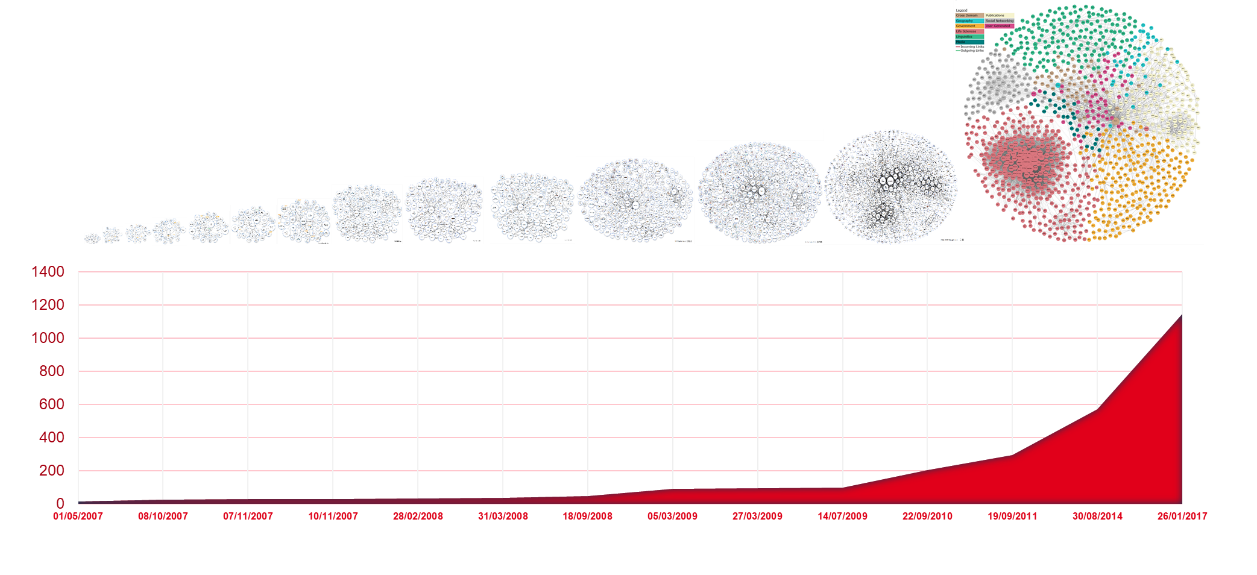
\includegraphics[width=5.0in]{media/image1.png}
    \caption{number of linked open datasets on the Web in the linked open
data cloud}
    \label{fig:ch1.1}
\end{figure}


\subsubsection{What about the round-worlders?}

The network effect has already proven to be an effective and empowering
way to muster the effort needed to create a massive information network
like the World Wide Web; in fact, it is the only method that has
actually succeeded in creating such a structure. The AAA slogan enables
the network effect that made the rapid growth of the Web possible. But
what are some of the ramifications of such an open system? What does the
AAA slogan imply for the content of an organically grown web?

For the network effect to take hold, we have to be prepared to cope with
a wide range of variance in the information on the Web. Sometimes the
differences will be minor details in an otherwise agreed-on area; at
other times, differences may be essential disagreements that drive
political and cultural discourse in our society. This phenomenon is
apparent in the hypertext web today; for just about any topic, it is
possible to find web pages that express widely differing opinions about
that topic. The ability to disagree, and at various levels, is an
essential part of human discourse and a key aspect of the Web that makes
it successful. Some people might want to put forth a very odd opinion on
any topic; someone might even want to postulate that the world is round,
while others insist that it is flat. The infrastructure of the Web must
allow both of these (contradictory) opinions to have equal availability
and access.

There are a number of ways in which two speakers on the Web may
disagree. We will illustrate each of them with the example of the status
of Pluto as a planet:


\begin{itemize}
\item
  \emph{They may fundamentally disagree on some topic}. While the IAU
  has changed its definition of planet in such a way that Pluto is no
  longer included, it is not necessarily the case that every astronomy
  club or even national body agrees with this categorization. Many
  astrologers, in particular, who have a vested interest in considering
  Pluto to be a planet, have decided to continue to consider Pluto as a
  planet. In such cases, different sources will simply disagree.
\item
  \emph{Someone might want to intentionally deceive}. Someone who
  markets posters, models, or other works that depict nine planets has a
  good reason to delay reporting the result from the IAU and even to
  spreading uncertainty about the state of affairs.
\item
  \emph{Someone might simply be mistaken}. Web sites are built and
  maintained by human beings, and thus they are subject to human error.
  Some web site might erroneously list Pluto as a planet or, indeed,
  might even erroneously fail to list one of the eight ``nondwarf''
  planets as a planet.
\item
  \emph{Some information may be out of date}. There are a number of
  displays around the world of scale models of the solar system, in
  which the status of the planets is literally carved in stone; these
  will continue to list Pluto as a planet until such time as there is
  funding to carve a new description for the ninth object. Web sites are
  not carved in stone, but it does take effort to update them; not
  everyone will rush to accomplish this.
\end{itemize}


While some of the reasons for disagreement might be, well, disagreeable
(wouldn't it be nice if we could stop people from lying?), in practice
there isn't any way to tell them apart. The infrastructure of the Web
has to be able to cope with the fact that information on the Web will
disagree from time to time and that this is not a temporary condition.
It is in the very nature of the Web that there be variations and
disagreement.

The Semantic Web is often mistaken for an effort to make everyone agree
on a single ontology--- but that just isn't the way the Web works. The
Semantic Web isn't about getting everyone to agree, but rather about
coping in a world where not everyone will agree and achieving some
degree of interoperability anyway. In the data themselves too we may
find disagreement; for instance the numbers of casualties in a conflict
may be reported on the Web of data with very different values from the
involved parties. There will always be multiple ontologies and diverging
statements, just as there will always be multiple web pages on any given
topic. The Web is innovative because it allows all these multiple
viewpoints to coexist.

\subsubsection{To each their own}

How can the Web architecture support this sort of variation of opinion?
That is, how can two people say different things, about the same topic?
There are two approaches to this issue. First, we have to talk a bit
about how one can make any statement at all in a web context.

The IAU can make a statement in plain English about Pluto, such as
``Pluto is a dwarf planet,'' but such a statement is fraught with all
the ambiguities and contextual dependencies inherent in natural
language. We think we know what ``Pluto'' refers to, but how about
``dwarf planet''? Is there any possibility that someone might disagree
on what a ``dwarf planet'' is? How can we even discuss such things?

The first requirement for making statements on a global web is to have a
global way of identifying the entities we are talking about. We need to
be able to refer to ``the notion of Pluto as used by the IAU'' and ``the
notion of Pluto as used by the American Federation of Astrologers'' if
we even want to be able to discuss whether the two organizations are
referring to the same thing by these names.

In addition to Pluto, another object was also classified as a ``dwarf
planet.'' This object is sometimes known as UB313 and sometimes known by
the name Xena. How can we say that the object known to the IAU as UB313
is the same object that its discoverer Michael Brown calls ``Xena''?

One way to do this would be to have a global arbiter of names decide how
to refer to the object. Then Brown and the IAU can both refer to that
``official'' name and say that they use a private ``nickname'' for it.
Of course, the IAU itself is a good candidate for such a body, but the
process to name the object took over two years. Coming up with good,
agreed-on global names is not always easy business.

On the Web we name things with URIs (Uniform Resource Identifier). The
URI standard provides rules to mint identifiers for anything around us.
The most common form of URIs are the URLs (Uniform Resource Locator)
commonly called Web addresses (e.g. http://www.inria.fr/) that locate a
specific resource on the Web. In the absence of an agreement, different
Web authors will select different URIs for the same real-world resource.
Brown's \emph{Xena} is IAU's \emph{UB313}. When information from these
different sources is brought together in the distributed network of
data, the Web infrastructure has no way of knowing that these need to be
treated as the same entity. The flip side of this is that we cannot
assume that just because two URIs are distinct, they refer to distinct
resources. This feature of the Semantic Web is called the Non-unique
Naming Assumption; that is, we have to assume (until told otherwise)
that some Web resource might be referred to using different names by
different people. It's also crucial to note that there are times when
unique names might be nice, but it may be impossible. Some other
organization than the IAU, for example, might decide they are unwilling
to accept the new nomenclature.

\subsubsection{There's always one more}
\label{openworld}

In a distributed network of information, as a rule we cannot assume at
any time that we have seen all the information in the network, or even
that we know everything that has been asserted about one single topic.
This is evident in the history of Pluto and UB313. For many years, it
was sufficient to say that a planet was defined as ``any object of a
particular size orbiting the sun.'' Given the information available
during that time, it was easy to say that there were nine planets around
the sun. But the new information about UB313 changed that; if a planet
is defined to be any body that orbits the sun of a particular size, then
UB313 had to be considered a planet, too. Careful speakers in the late
twentieth century, of course, spoke of the ``known'' planets, since they
were aware that another planet was not only possible but even suspected
(the so-called ``Planet X,'' which stood in for the unknown but
suspected planet for many years).

The same situation holds for the Semantic Web. Not only might new
information be discovered at any time (as is the case in solar system
astronomy), but, because of the networked nature of the Web, at any one
time a particular server that holds some unique information might be
unavailable. For this reason, on the Semantic Web we can rarely conclude
things like ``there are nine planets,'' since we don't know what new
information might come to light.

In general, this aspect of a Web has a subtle but profound impact on how
we draw conclusions from the information we have. It forces us to
consider the Web as an Open World and to treat it using the Open World
Assumption. An Open World in this sense is one in which we must assume
at any time that new information could come to light, and we may draw no
conclusions that rely on assuming that the information available at any
one point is all the information available.

For many applications, the Open World Assumption makes no difference; if
we draw a map of all the Mongotel hotels in Boston, we get a map of all
the ones we know of at the time. The fact that Mongotel might have more
hotels in Boston (or might open a new one) does not invalidate the fact
that it has the ones it already lists. In fact, for a great deal of
Semantic Web applications, we can ignore the Open World Assumption and
simply understand that a semantic application, like any other web page,
is simply reporting on the information it was able to access at one
time.

The openness of the Web only becomes an issue when we want to draw
conclusions based on distributed data. If we want to place Boston in the
list of cities that are not served by Mongotel (e.g., as part of a
market study of new places to target Mongotels), then we cannot assume
that just because we haven't found a Mongotel listing in Boston, no such
hotel exists.

As we shall see in the following chapters, the Semantic Web includes
features that correspond to all the ways of working with Open Worlds
that we have seen in the real world. We can draw conclusions about
missing Mongotels if we say that some list is a comprehensive list of
all Mongotels. We can have an anonymous ``Planet X'' stand in for an
unknown but anticipated entity. These techniques allow us to cope with
the Open World Assumption in the Semantic Web, just as they do in the
Open World of human knowledge.

In contrast to the Open World Assumption, most data systems operate under the
\emph{Closed World Assumption}, that is, if we are missing some data in a document or a record,
then that data is simply not available.  In many situations (such as when evaluating
documents that have a set format or records that conform to a particular data base schema),
the Closed World Assumption is appropriate.   The Semantic Web standards have provisions for
working with the Closed World Assumption when it is appropriate. 


\subsubsection{The nonunique name of the semantic Web}

One problem the first time you discover linked data on the Web and
semantic Web is that this evolution of the Web is perceived and
presented under different names, each name insisting on a different
facet of the overall architecture of this evolution. In the title of
this book, we refer to the Semantic Web, emphasizing the importance of
meaning to data sharing. The Semantic Web is known by many other names.
The name ``Web of data'' refers to the opportunity now available on the
Web to open silos of data of all sizes, from the small dataset of a
personal hotel list up to immense astronomic databases, and to exchange,
connect and combine them on the Web according to our needs. The name
``linked data'' refers to the fact we can use the Web addressing and
linking capabilities to link data pieces inside and between datasets
across the Web much in the same way we reference and link Web pages on
the hypertext Web. Only this time, because we are dealing with structured
data, applications can process these data and follow the links to
discover new data in many more automated ways. The name ``linked open
data'' focuses on the opportunity to exploit open data from the Web in
our applications and the high benefit there is in using and reusing URIs
to join assertions from different sources. This name also reminds us
that linked data are not necessarily open and that all the techniques we
are introducing here can also be used in private spaces (intranets,
intrawebs, extranets, etc.). In an enterprise, we often refer to a
``Knowledge Graph'', which is specific to that enterprise, but can
include any information that the enterprise needs to track (including
information about other enterprises that it does business with). The
name ``giant global graph'' puts into perspective the billions of links
between data distributed on the Web and which, joined through URIs,
produce a giant graph. The name ``semantic web'' emphasizes the ability
we now have for exchanging our data models, schemas, vocabularies, in
addition to datasets, and the associated semantics in order to enrich
the range of automatic processing that can be performed on them as we
will see in Chapter~\ref{ch7}.

\section{SUMMARY}

The aspects of the Web we have outlined here---the AAA slogan, the
network effect, nonunique naming, and the Open World
Assumption---already hold for the hypertext Web. As a result, the Web
today is something of an unruly place, with a wide variety of different
sources, organizations, and styles of information. Effective and
creative use of search engines is something of a craft; efforts to make
order from this include community efforts like social bookmarking and
community encyclopedias to automated methods like statistical
correlations and fuzzy similarity matches.

For the Semantic Web, which operates at the finer level of individual
statements about data, the situation is even wilder. With a human in the
loop, contradictions and inconsistencies in the hypertext Web can be
dealt with by the process of human observation and application of common
sense. With a machine combining information, how do we bring any order
to the chaos? How can one have any confidence in the information we
merge from multiple sources? If the hypertext Web is unruly, then surely
the Semantic Web is a jungle---a rich mass of interconnected
information, without any road map, index, or guidance.

How can such a mess become something useful? That is the challenge that
faces the working ontologist. Their medium is the distributed web of
data; their tools are the Semantic Web languages RDF, RDFS, SPARQL,
SKOS, SHACL and OWL. Their craft is to make sensible, usable, and
durable information resources from this medium. We call that craft
modeling, and it is the centerpiece of this book.

The cover of this book shows a system of channels with water coursing
through them. If we think of the water as the data on the Web, the
channels are the model. If not for the model, the water would not flow
in any systematic way; there would simply be a vast, undistinguished
expanse of water. Without the water, the channels would have no
dynamism; they have no moving parts in and of themselves. Put the two
together, and we have a dynamic system. The water flows in an orderly
fashion, defined by the structure of the channels. This is the role that
a model plays in the Semantic Web.

Without the model, there is an undifferentiated mass of data; there is
no way to tell which data can or should interact with other data. The
model itself has no significance without data to describe it. Put the
two together, however, and you have a dynamic web of information, where
data flow from one point to another in a principled, systematic fashion.
This is the vision of the Semantic Web---an organized worldwide system
where information flows from one place to another in a smooth but
orderly way.

\subsection{Fundamental concepts}

The following fundamental concepts were introduced in this chapter.

\textbf{The AAA slogan}---Anyone can say Anything about Any topic. One
of the basic tenets of the Web in general and the Semantic Web in
particular.

\textbf{Open world/Closed world}---A consequence of the AAA slogan is
that there could always be something new that someone will say; this
means that we must assume that there is always more information that
could be known.

\textbf{Nonunique naming}---Since the speakers on the Web won't
necessarily coordinate their naming efforts, the same entity could be
known by more than one name.

\textbf{The network effect}---The property of a web that makes it grow
organically. The value of joining in increases with the number of people
who have joined, resulting in a virtuous cycle of participation.

\textbf{The data wilderness}---The condition of most data on the web. It
contains valuable information, but there is no guarantee that it will be
orderly or readily understandable.



